\chapter{Datenstrukturen}

Im Allgemeinen haben wir zwei Anforderungen an die verwendeten Datenstrukturen, welche zur Repräsentation der Graphen verwendet werden: Es muss möglich sein für einen Knoten seine Vorgänger und Nachfolger zu finden und es muss möglich sein Kanten zu verändern oder zu entfernen.
Diese beiden Ansprüche stehen sich mitunter gegenüber.

Sollange nicht anders erwähnt, wurden für

Vertices sind natürliche Zahlen bzw uint32.
Ein Graph enthält idealerweise keine isolierten Knoten.
isolierte Knoten sind doof für dijkstra und co.
Die Menge der Knoten ist definiert durch Ihre Anzahl.
Gibt es $n \in \mathbb{N}$ Knoten, so sind es $0, \dotsc, n - 1$.
Ein Graph der diese Eigenschaft nicht erfüllt, kann durch eine Mapping der Knoten in die Form gebracht werden.

Jenachdem was mit dem Graph gemacht werden soll, sind verschiedene Eigenschaften von Vorteil.
Manchmal ist eine effiziente Nachbar Abfrage wichtig,
Manchmal das bearbeiten des Graphes, einfügen oder löschen von Knoten

Es wurde ein dyn Trait benutzt, welches eine Overhead hat und kein inlining zulässt.
Dafür lassen sich verschiedene Methoden vergleichen.

Die Grundlegenden Implementierungen kennen nur ihre Vorgänger.
Ein Reversibe Graph besteht aus einem Graph und seinem Umkehrgraph.
Gleiche Datenstruktur.

\subsection{VecVecGraph}
Ein Vec mit pro Knoten ein Vec.
Der innere Vec speichert Tuple aus (Vertex, Distanz).
Der innere Vec ist nach Vertex sortiert.

Ein Knoten kann so mit eine binären Suche gefunden werden.
Doch ab einem großen Grad wird diese Suche teuer.
Das einfügen und Löschen ist auch etwas teuere, da die übrigen Elemente geschoben werden müssen

Das finden von Nachbarn geht aber schnell, weil kein unbenutzer Platz dazwischen ist.

\subsection{VecHashMap}
Ein Vec mit pro Knoten eine HashMap
Die innere HashMap speichert Vertex -> Distanz.
So kann schnell ein Knoten gefunden werden.

Das finden von Nachbarn ist etwas langsamer, da unbenutzter Platz zwischen den Hash Einträgen.

Das einfügen und löschen ist günstig.

Vielleicht wäre IndexMap noch spannend.
Schnelles finden von Nachbarn.
Schnelles Iterieren.

Einfügen und löschen etwas teuerer.

\subsection{VecGraph}
Zwei Vecs.
Ein Index Vec mit pro Knoten ein Eintrag (u32, u32).
Dieser Eintrag gibt den Startindex und Stopindex des des zweiten Vecs an.
Dieser ist ein Vec (Vertex, Distanz).

Das bietet den Vorteil, dass man die Kanten zusätzlich sortieren kann, für besser Cache lokalität.
Kanten häufig benutzter Knoten können so an einem Ende des Vec grupiert werden.

\chapter{CH Bruteforce}

Wie zu sehen sein wird, lässicht sich die klassischen Methode zur Erstellung der benötigten Datenstrukturen nur bedingt auf Sichtbarkeitsgraphen anwenden.
Daher wird im follgenden zuerst unabhängig von der Erstellung argumentiert um später mehre Methoden hierfür vorzustellen.

Contraction Hierarchies bauen auf der Notation eines \emph{Levels} auf, jedem Knoten wird ein Level zugeorndet.
Diese kann als ein Grad der Wichtigkeit verstanden werden:
Je höher ein Level ist, desto wichtiger ist der Knoten im Allgemeinen für das Finden von kürzesten Pfaden.

\begin{definition}[Level]
    Sei $G = (V, E)$ ein Graph.
    Sei $L \subseteq \mathbb{N}$ mit $\abs{L} = \abs{V}$.
    Dann wird eine bijketive Funktion ${vtl} \coloneq V \to L$ \emph{vertex-to-level} Funktion genannt.
    Ihre Umkehrfunktion ${ltv}$ wird \emph{level-to-vertex} Funktion genannt.
\end{definition}

Die ein Level aus genau einem Knoten besteht, ist keine zwingen Notwendigkeit
So setzt \cite{vetter2009parallel} etwa mehrere Knoten auf einem Level, um das Preprocessing zu beschleunigen.
Die in dieser Arbeit verwende Einschränkung vereinfacht allerdings die Argumentation.

Bassierend auf dem Level kann der \emph{upward Graph} definiert werden.
Formal ist dieser definiert als:

\begin{definition}[Upward Graph]
    Sei $G = (V, E)$ und ${vtl}$ eine \emph{vertex-to-level} Funktion dazu. Dann ist $G_u = (V, E_u)$ ein \emph{upward Graph} zu $G$ wenn gilt:
    \begin{enumerate}
        \item\label{ch:definition:legal_edges}
        $E_u$ enthält nur Kanten $(t, h, d)$ mit $t, h \in V$ und $d \in \mathbb{R}^+$, für die gillt, $d \geq {spd}_{G}((t, h))$ und es einen $(t, h)$ Pfad gibt, so dass $h$ das größte und $t$ das zweitgrößte Level auf diesem hat.

        \item\label{ch:definition:upward}
        $E_u$ enthält mindestens alle Kanten $(t, h, {spd}_{G}((t, h)))$ mit $t, h \in V$, für die gilt, dass $h$ das größte und $t$ das zweitgrößte Level auf allen kürzesten Wege auf $G$ von $t$ nach $h$ hat.
    \end{enumerate}
\end{definition}


Betrachten wir das ganze an dem bereits definierten Beispielgraph.
Sei ${vtl}$ definiert durch die Abbildung in \autoref{ch::fig::vtl_abbildung} definiert.
Durch Anwendung der Regel \ref{ch:definition:upward} ergibt sich der in \autoref{ch::fig::upward_graph} gezeigte upward Graph.
Es ist hierbei zu erwähnen, dass keine zusätzlichen Kanten nach \autoref{ch:definition:legal_edges} eingefügt wurden.

Der enstande Graph ist azyklisch, da er nur Kanten enthält, deren Kopf ein größeres Level als ihr Fuß hat.
Die Anzahl der in einer Breitensuche gefunden Knoten ist geringer, als im Ursprungsgraph.
Diese beiden Eingeschaften sorgen dafür, dass eine Suche in einem upward Graph kostengünstiger sei kann.
Die in einem upward Graph gefunden kürzesten Pfade bilden eine untere Grenze für kürzeste Pfade.

\begin{table}[ht]
    \centering
    \begin{tabular}{lllllllllllll}
        Vertex & a & b & c & d & e & f & g & h & i & j  & k & \\
        Level  & 8 & 7 & 3 & 6 & 2 & 5 & 1 & 4 & 0 & 10 & 9 &
    \end{tabular}
    \caption{${vtl}$ Beispielfunktion}
    \label{ch::fig::vtl_abbildung}
\end{table}


\begin{figure}[ht]
    \centering
    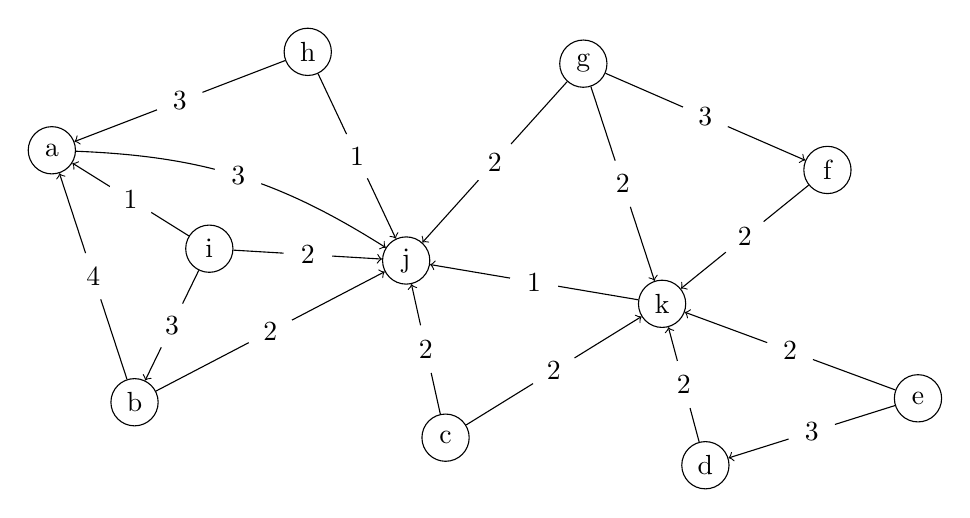
\begin{tikzpicture}
        % Nodes
        \node[circle, draw, minimum size=0.6cm, inner sep=0pt] at (0.5* 0.0, 0.5* 8.5)  (a)    {a};
        \node[circle, draw, minimum size=0.6cm, inner sep=0pt] at (0.5* 2.1, 0.5* 2.1)  (b)    {b};
        \node[circle, draw, minimum size=0.6cm, inner sep=0pt] at (0.5* 10.0, 0.5* 1.2)  (c)    {c};
        \node[circle, draw, minimum size=0.6cm, inner sep=0pt] at (0.5* 16.6, 0.5* 0.5)  (d)    {d};
        \node[circle, draw, minimum size=0.6cm, inner sep=0pt] at (0.5* 22.0, 0.5* 2.2)  (e)    {e};
        \node[circle, draw, minimum size=0.6cm, inner sep=0pt] at (0.5* 19.7, 0.5* 8.0)  (f)    {f};
        \node[circle, draw, minimum size=0.6cm, inner sep=0pt] at (0.5* 13.5, 0.5* 10.7)  (g)    {g};
        \node[circle, draw, minimum size=0.6cm, inner sep=0pt] at (0.5* 6.5, 0.5* 11.0)  (h)    {h};
        \node[circle, draw, minimum size=0.6cm, inner sep=0pt] at (0.5* 4.0, 0.5* 6.0)  (i)    {i};
        \node[circle, draw, minimum size=0.6cm, inner sep=0pt] at (0.5* 9.0, 0.5* 5.7)  (j)    {j};
        \node[circle, draw, minimum size=0.6cm, inner sep=0pt] at (0.5* 15.5, 0.5* 4.6)  (k)    {k};


        \draw[->]  (a) edge[bend left=15] node[circle, fill=white] {3} (j);

        \draw[->]  (b) edge node[circle, fill=white] {4} (a);
        \draw[->]  (b) edge node[circle, fill=white] {2} (j);

        \draw[->]  (c) edge node[circle, fill=white] {2} (j);
        \draw[->]  (c) edge node[circle, fill=white] {2} (k);

        \draw[->]  (d) edge node[circle, fill=white] {2} (k);

        \draw[->]  (e) edge node[circle, fill=white] {3} (d);
        \draw[->]  (e) edge node[circle, fill=white] {2} (k);

        \draw[->]  (f) edge node[circle, fill=white] {2} (k);

        \draw[->]  (g) edge node[circle, fill=white] {3} (f);
        \draw[->]  (g) edge node[circle, fill=white] {2} (j);
        \draw[->]  (g) edge node[circle, fill=white] {2} (k);

        \draw[->]  (h) edge node[circle, fill=white] {3} (a);
        \draw[->]  (h) edge node[circle, fill=white] {1} (j);

        \draw[->]  (i) edge node[circle, fill=white] {1} (a);
        \draw[->]  (i) edge node[circle, fill=white] {3} (b);
        \draw[->]  (i) edge node[circle, fill=white] {2} (j);


        \draw[->]  (k) edge node[circle, fill=white] {1} (j);
    \end{tikzpicture}
    \caption{Upward Graph des Beispielgraphs}
    \label{ch::fig::upward_graph}
\end{figure}

Die Suche eines kürzesten Pfades ist dann eine bidirectionale Suche, wobei die Suchen auf verschiedenen Graphen arbeiten.
Daher muss noch das Gegenstück das upward Graphens definiert werden, der \emph{downard Graph}.

\begin{definition}[Downward Graph]
    Sei $G = (V, E)$ und ${vtl} \coloneq V \to \mathbb{N}$ eine \emph{vertex-to-level} Funktion. Dann ist ein upward Graph des Umkehrgraphens $G^T$ ein \emph{downward Graph} zu $G$.
\end{definition}

Wenn ein Graph ungerichtet ist, dann ist er äuivalent zu seinem Umkehrgraphen und dann ist auch der Upward und Downward Graph äuivalent.
Daher entspricht \autoref{ch::fig::upward_graph} gleichzeitig auch dem Downward Graph des Beispielgraphens.


\subsubsection{Ideen}

Die bisher erwähnten Methoden eignen sich nur bedingt für Graphen mit großem durchscnittlichen Knotengrad.
Dieser wirkt sich auf die Erstellungzeit der Kanten-Differenz, da für jedes Paar aus Vorgänger und Nachfolger geprüft werden muss, ob bereits eine Kante zwischen ihnen exisitert.
Auch wenn dies durch eine passende Datenstruktur sehr effizient geschehen kann, kann dies sehr teuer sein:
Angenommen ein Knoten hat einen Grad von \num{10000}, dann müssen \num{100000000} viele Paare geprüft werden.
Bei einer angenommen Suchzeit von \num{10}\unit{\ns} pro Paar entspricht dies einer Sekunde.


Daher gibt es zwei Baustellen, die beschleunigt werden müssen:
Die Heuristik und die Kontraktion.

\paragraph{Kontraktion}
Anstatt einer teuren Suche kann auch eine Heuristik verwendet werden, welche eine obere Schranke angibt.
Dies ist insofern auch nicht abwägig, da die abgeschwächte Dijkstra Suche selbst nur eine obere Schranke angibt.
Eine Abkürzung wird dann eingefügt, wenn ihre Länge kleiner gleich einer oberen Schranke ist.
Falls es günstiger ist untere Schranken zu ermitteln, kann auch zuerst geprüft werden, ob die Länge gleich einer unteren Schranke ist, dann muss ebenfalls eine Abkürzung eingefügt werden.

\subparagraph{Triviale Heurisik}
Eine mögliche Idee ist, jede mögliche Abkürzung einzufügen, also die obere Schranke $\infty$ zu wählen.
Unter der Annahme, dass bei einem sehr hohem Kantengrad fast alle Vorgänger bereits Kanten zu fast allen Nachfolgern haben, ist der Anteil der unötig eingefügenten Kanten zu den notwendig eingefügten Kanten vielleicht vertertbar.
Die Berechnung der Kanten-Differenz und der Kontraktion sind dabei ebenfalls gleich, was beim Lazy-Popping praktisch ist, da dann die neuberechnung der Heuristik ebenfalls die neuen Kanten liefert.

\subparagraph{Vereinfacher Graph}
Gibt es einen vereinfachten Graphen $G'$, der obere Schranken zu $G$ für alle Knotenpaare liefert, dann kann auf diesem gesucht werden.
Insbesondere kann eine auf $G'$ angwendet Speedup-Technik verwendet werden, wie etwe Contraction Hierarchies oder Hub Labels.

\subparagraph{Dreickunsgleichung}
Ähnlich zu ALT\cite{goldberg2005computing} kann eine Menge Landmarks berechnet werden, welche mittels der Dreiecksungleichung eine obere Schranke angeben können.
Ein Landmark ist hierbei ein Knoten, für den die Distanz zu und von allen Knoten bekannt ist.
Hierbei gilt für ein Landmark $l \in V$, dass für alle $u, v \in V$ mittels ${spd}((u, l)) + {spd}((l, u))$ eine obere Schranke bestimmt werden kann.
Liegt $l$ dabei auf einem kürzesten Pfad von $u$ nach $v$, so entspricht der Wert sogar genau dem der kürzesten Pfad Distanz.
Damit durch ein möglichst kleine Menge an Landmarks eine möglichst große Menge an Pfaden abgeckt wird, müssen diese ein Hitting Setüber eine möglichst große Menge an Pfaden bilden.

Die Methoden der Dreicksungleichung und des Vereinfachten Graphens können auch kombiniert werden, wobei die jeweils kleinere obere Schranke ausgewählt wird.
Die Hoffnung hierbei ist, dass der Vereinfachte Graph Kanten mit einem niedrigen Hop-Abstand gut abschätzen kann, die Dreiecksungleichung gut Pfade mit einem hohen Hop Abstand, da die Wahrscheinlichkeit dass ein Landmark auf oder nahe einem kürzesten Pfad ist dann steigt.

\paragraph{Propabalistische Heuristik}
Wie bereits erwähnt wird bei großen Kantengraden die Berechnung der Kanten-Differenz sehr teuer.
Eine Idee diese Kosten anzufangen, ist es die Kanten-Differenz heuristisch anzuhnähern.
Dafür wird eine Teilmenge aller Vorgänger, Nachfolgerpaare gebildet für die die Kanten-Differenz gebildet wird.
Dieses Ergebnis wird dann auf die tatsächliche Menge an Paaren skaliert.
Dies kann nicht ohne weiteres mit Lazy Popping zusammen verwendet werden, da sich das die Ergebnisse bei zwei aufraufen hinterinander unterscheiden kann.
Dies kann dazu führen, dass unötigt oft Lazy gepoppt wird.

\paragraph{Layz Popping}
Bei normalen Lazy Popping wird ein Knoten zurückgepusht, wenn er nicht mehr den gleichen Heuristik-Wert wie zuvor hat.
Dies könnte angepasst werden, so dass ein gewisse Abweichung, entweder absolut oder relativ, zulässig ist.

\paragraph{Neighbor update}
Anstatt jeden Nachbar sofor upzudaten kann für jeden Nachbarn mitgezählt werden, wie oft ein Nachbar kontraktiert wurde.
Erst wenn dies einen gewissen Schwellwert überschritten hat, wird der Knoten geupdated.

\paragraph{Neubrechnung alle $n$ kontraktionen}
Die Heuristik-Werte werden all $n$ Kontraktionen für alle Knoten neuberechnet.

\section{Brute force}

Die in der Defintion des upward Graphens genannten Kanten könnne auch berechnet werden, indem für jede Graphe eine angepasste Dijkstra Suche durchgeführt wird.
Dafür wird während der Dijstra Suche notiert, was das größte Level auf dem Weg von der Wurzel bis zu dem Knoten ist.
Ein Knoten ist der Kopf eine CH Kante, für die gilt, dass das größte Level auf dem Weg zur Wurzel zu ihr sie selber hat und der größte Level des Vorgängers der der Wurzel ist.
Das Gewicht der Kante kann Dijkstra entommen werden.

Während es für Straßengraphen vermutlich deutlich teuer ist, kann es für ander Graphenklassen durchaus Sinn machen, wenn andere Methoden zur Erstellung eines Contracted Graphen noch teuerer sind.
Die Berechung ist \emph{embarrassingly parallel}, da jeder Knoten für sich selbst Berechnet werden kann, wobei das Erstellen der Abkürzungen, sofern benötigt, synchronisert werden sollte, um den Speichbedarf zu verkleinern.

\todo{Ich habe die Vermutung, dass theoretisch die Laufzeit pro Knoten für Bruteforce immer größer gleich all-in ist}

\subsection{Alogrithmus im Detail}

Betrachten wir wieder eine Suche vom Knoten $a$ im Beispielgraphen.
Ihr Suchbaum ist \autoref{ch:fig:brute_force_suchbaum} gezeigt.
Die Höhe der Knoten entspricht hierbei dem Zeitpunkt der Expansion, die linke Zahl steht für das dem Knoten zugewiesene Level, die rechte für das höchste Level auf dem Weg zzur Wurzel.
Die Definition des upward Graphens besagt, dass genau dann eine Kante $(u, v)$ eingefügt werden muss, wenn ${vtl}(v) > {vtl}(v)$ und es auf allen kürzesten Pfaden zwischen $v$ den höchsten und $u$ den zweithöchsten Level hat.
Für die Berechnung schwächen wir dies ab, und fügen eine Kante ein, wenn es einen kürzesten Pfad gibt, der dies erfüllt.
Hierfür tracken wir den höchsten Level, welcher auf dem Weg von der Wurzel zum Knoten bisher gesehen wurde.
Der erste Knoten auf dem jedem Weg von der Wurzel zum Blatt, für den gilt, dass er selbst das größte Level hat, bildet den Kopf einer Kante im upward Graph.


Die Suche muss dabei nicht bis zum Ende durchgeführt werden.
Es reicht so lange zu suchen, bis es keine Knoten mehr gibt, die noch nicht expandiert wurden und für die es auf dem Weg zur Wurzel nicht mindestens eine solche Kante gibt.
Hierfür wird eine Menge an \emph{lebendigen} Knoten benutzt.
Zu beginn ist nur der Startknoten lebendig, die Lebendigkeit wird jeweils an die Kinder vererbt.
Ein Knoten stirbt, nachdem er expandiert wurde oder wenn er den Kopf einer Kante bildet.
Gibt es keine lebendigen Knoten mehr, so kann die Suche abgebrochen werden.
In dem verwendeten Beispiel wäre dies etwa nach der Expansion von $b$ der Fall.


% \begin{algorithm}[ht]
%     \caption{Contracted Graph Brute Force Suchalgorithmus}
%     \begin{algorithmic}[1]
%         \Require Graph $G = (V, E)$, vertex-to-level Funktion ${vtl}$, Startknoten $s \in V$, Zielknoten $t \in V$
%         \Ensure $E_s$
%         \State // Initialisiere Distanz- und Vorgänger-Funktion
%         \ForAll{$v \in V$}
%         \State ${dist}(v) \leftarrow \infty$
%         \State ${pre}(v) \leftarrow {none}$
%         \EndFor
% 
% 
%         \State
%         \State // Initialisiere Vorrangwarteschlange
%         \State ${dist}(s) \leftarrow 0$
%         \State $Q\leftarrow \{ s \}$
% 
% 
%         \State
%         \State // Initialisiere max\_level\_path
%         \State ${mlp}(s) \leftarrow {vtl}(s)$
%         \State $E_s \leftarrow \{ \}$
%         \State ${alive} \leftarrow \{ s \}$
% 
%         \State
%         \While{$Q \neq \emptyset \land {alive} \neq \emptyset$}
%         \State $u \leftarrow{extract\_min}(Q)$\label{graphs:dijkstra:pop}
% 
%         \State
%         \State // Beende frühzeitig wenn Zielknoten gefunden wurde
%         \If {$u \neq s \land {mlp}(u) = {vtl}(u)$}
%         \State $E_s \leftarrow E_s \cup \{ (s, u, {dist}(u)) \}$
%         \State ${alive} \leftarrow {alive} \setminus \{ s \}$
%         \EndIf
% 
%         \State
%         \State // Aktualisiere Nachbarn
%         \ForAll{$(u, v, w) \in E$}
%         \If {${dist}(u) + w < {dist}(v)$}
%         \State ${dist}(v) \leftarrow {dist}(u) + w$
%         \State ${pre}(u) \leftarrow v$
%         \State $Q = Q \cup \{ v \}$
%         \State
%         \State // setze max\_level\_path
%         \State ${mlp}(v) \leftarrow \max({mlp}(v), {vtl}(v))$
%         \If {$u \in {alive}$}
%         \State ${alive} \leftarrow {alive} \cup \{ s \}$
%         \EndIf
%         \EndIf
%         \EndFor
% 
% 
%         \State ${alive} \leftarrow {alive} \setminus \{ s \}$
% 
%         \EndWhile
% 
%         \State
%         \State \Return $E_s$
%     \end{algorithmic}
% \end{algorithm}

\begin{figure}[ht]
    \centering
    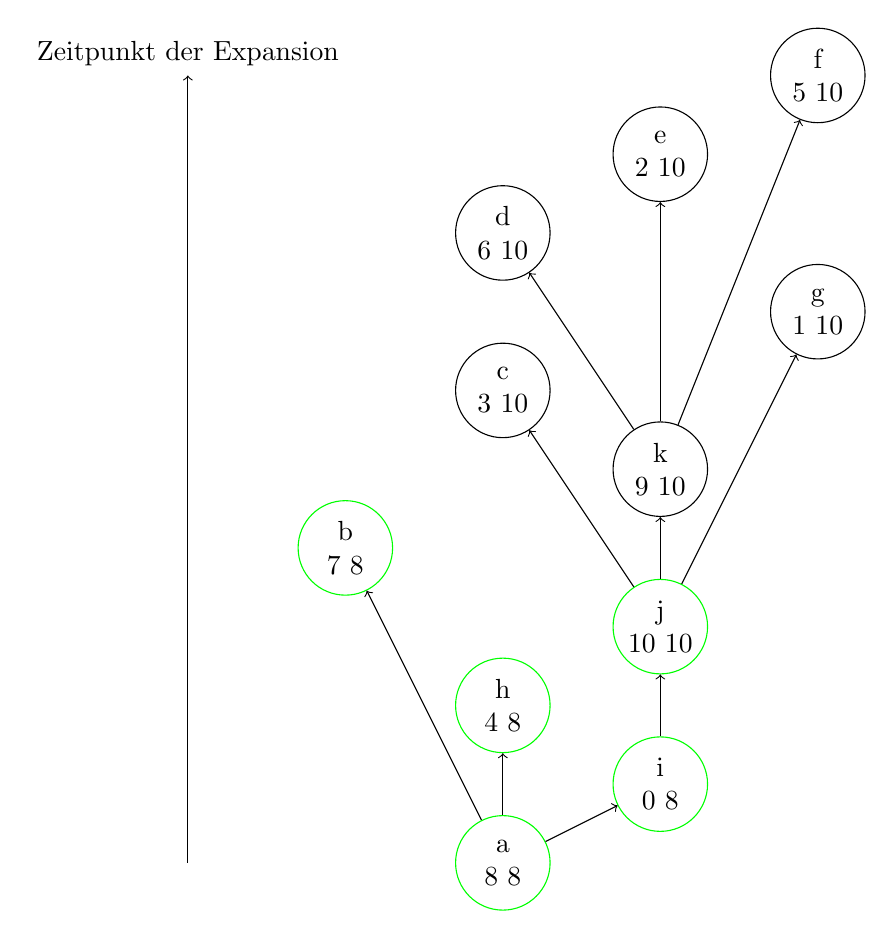
\begin{tikzpicture}
        % Nodes
        % a & b & c & d & e & f & g & h & i & j & k & 
        % 8 & 7 & 3 & 6 & 2 & 5 & 1 & 4 & 0 & 10 & 9 & 

        \node[circle, draw=green, minimum size=1.2cm, inner sep=0pt , align=center] at (2* 1, 0)  (a)    {a\\8 8};
        \node[circle, draw=green, minimum size=1.2cm, inner sep=0pt , align=center] at (2* 0, 4)  (b)    {b\\7 8};
        \node[circle, draw, minimum size=1.2cm, inner sep=0pt , align=center] at (2* 1, 6)  (c)    {c\\3 10};
        \node[circle, draw, minimum size=1.2cm, inner sep=0pt , align=center] at (2* 1, 8)  (d)    {d\\6 10};
        \node[circle, draw, minimum size=1.2cm, inner sep=0pt , align=center] at (2* 2, 9)  (e)    {e\\2 10};
        \node[circle, draw, minimum size=1.2cm, inner sep=0pt , align=center] at (2* 3, 10)  (f)    {f\\5 10};
        \node[circle, draw, minimum size=1.2cm, inner sep=0pt , align=center] at (2* 3, 7)  (g)    {g\\1 10};
        \node[circle, draw=green, minimum size=1.2cm, inner sep=0pt , align=center] at (2* 1, 2)  (h)    {h\\4 8};
        \node[circle, draw=green, minimum size=1.2cm, inner sep=0pt , align=center] at (2* 2, 1)  (i)    {i\\0 8};
        \node[circle, draw=green, minimum size=1.2cm, inner sep=0pt , align=center] at (2* 2, 3)  (j)    {j\\10 10};
        \node[circle, draw, minimum size=1.2cm, inner sep=0pt , align=center] at (2* 2, 5)  (k)    {k\\9 10};


        \draw[->]  (a) edge (b);
        \draw[->]  (a) edge (h);
        \draw[->]  (a) edge (i);
        \draw[->]  (j) edge (c);
        \draw[->]  (i) edge (j);
        \draw[->]  (k) edge (d);
        \draw[->]  (j) edge (k);
        \draw[->]  (k) edge (e);
        \draw[->]  (k) edge (f);
        \draw[->]  (j) edge (g);

        \draw[->] (-2, 0) -- (-2, 10) node[above] {Zeitpunkt der Expansion};

    \end{tikzpicture}
    \caption{Brute-Force Suche}
    \label{ch:fig:brute_force_suchbaum}
\end{figure}

\subsection{Abkürzung Problem}

Es liegt nahe als abgekürzten Knoten den Knoten mit dem dritthöchsten Level auszuwählen und sich darauf zu verlassen, dass die Suche von diesem Knoten aus die nächsen Abkürzung findet, und so weiter.
Dies wäre praktisch, da dann jeder Shortcut nur einmal erstellt werden müsste.
Zwei Gründe können jedoch dagegen sprechen:
Wird als Graph eine Datenstruktur verwendet, welche die Nachbarn nicht in einer definierten Ordnung ausgibt (etwa ein Hashset), können zwei Suchen von bzw. zu einem Knoten zwei Unterschiedliche kürzeste Pfad Bäume bilden.
Eine nicht stabile Prioritätswarteschlange kann ebenfalls den gleichen Effekt herbeiführen.

\autoref{ch:fig:problem_shortcut} zeigt eine Situation, in der so ein Problem auftreten kann.
Für den Knoten $a$ wird die Kante $(a, e)$ mit dem abekürztem Knoten $d$ gefunden.
Wir verlassen uns darauf, dass die Suche von $d$ aus die Abkürzung $(d, a)$ mit dem Knotem $b$ findet.

Die Lösung hierfür ist, dass die Abkürzungen, welche benötigt werden, um die ursprüngliche Abkürzung vollständiz zu entpacken, ebenfalls erstellt werden.
Diese werden aber mit einer hohen Wahrscheinlichkeit von den Bruteforcing der jeweils abgekürzten Knoten endeckt.
Der Speichermehrbedarf hierbei kann ein Problem für die Umsetzbarkeit des Algorithmus werden, weshalb ein Mechanismus verwendet werden sollte, welcher die mehrfache Speicherung verhindet, etwa eine HashMap.
Dies führt allerdings zu einem Performance-Hit, da dies synchroniesert werden muss.
Für denn Fall, dass nur die kürzesten Pfad Abstände Interesannt sind, kann und sollte hierauf verzichtet werden.

\begin{figure}[ht]
    \centering

    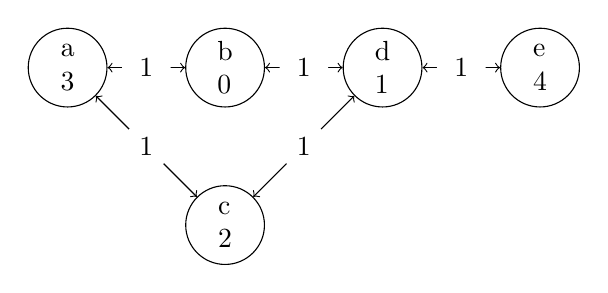
\begin{tikzpicture}
        % Nodes
        \node[circle, draw, minimum size=1cm, inner sep=0pt, align=left] at (2*0, 2*0)  (a)    {a\\3};
        \node[circle, draw, minimum size=1cm, inner sep=0pt, align=left] at (2*1, 2*0)  (b)    {b\\0};
        \node[circle, draw, minimum size=1cm, inner sep=0pt, align=left] at (2*1, 2*-1)  (c)    {c\\2};
        \node[circle, draw, minimum size=1cm, inner sep=0pt, align=left] at (2*2, 2*0)  (d)    {d\\1};
        \node[circle, draw, minimum size=1cm, inner sep=0pt, align=left] at (2*3, 2*0)  (e)    {e\\4};


        \draw[<->]  (a) edge node[circle, fill=white] {1} (b);
        \draw[<->]  (b) edge node[circle, fill=white] {1} (d);
        \draw[<->]  (d) edge node[circle, fill=white] {1} (e);


        \draw[<->]  (a) edge node[circle, fill=white] {1} (c);
        \draw[<->]  (c) edge node[circle, fill=white] {1} (d);
    \end{tikzpicture}
    \caption{Problem beim Shortcut erstellen}
    \label{ch:fig:problem_shortcut}
\end{figure}

\chapter{HL Brute Froce}


\begin{definition}[Forward Label, Reverse Label]
    Sei $G = (V, E)$ und ${vtl}$ eine \emph{vertex-to-level} Funktion dazu. Dann ist die Menge $f_t \subseteq V \times \mathbb{R}$ ein \emph{forward Label} auf $G$ zu $t \in V$ wenn gilt:

    \begin{enumerate}
        \item
              Es gibt kein Knoten $v \in V$, welcher mit zwei verschiedenen Distanzen in $f_v$ ist.

        \item
              $f_v$ enthält nur $(h, d)$ mit $t \in V$, $d \in \mathbb{R}$ für die ${vtl}(h) > {vtl}(t)$ und $d \geq {spd}_G ((v, h))$ gilt.

        \item
              $f_v$ enthält alle $(h, d)$ mit $t \in V$, $d \in \mathbb{R}$ für die gilt, dass $d = {spd}_G ((v, h))$ und dass $h$ das größte Level auf allen kürzesten Wegen auf $G$ zur Wurzel hat.
    \end{enumerate}

    Analog dazu ist $r_t$ ein \emph{Reverse Label} ein Forward Label auf dem Umkehrgraphen $G^T$. Ist $G$ ungerichtet, so sind Forward Label und Reverse Label äuivalent.
\end{definition}

Dass besondere an diesen Labels ist, dass für eine ${vtl}$ Funktion es für jeden Kontenpaar $s, t \in V$, für die es einen kürzesten Pfad zwischen ihen gibt, ein Treffpunkt-Knoten $m \in V$ gibt, der im Forward und Reverse Label mit optimaler Distanz ist.

\chapter{Ergebnisse}


\begin{figure}[ht]
    \centering
    \begin{subfigure}[b]{0.35\textwidth}
        \centering
        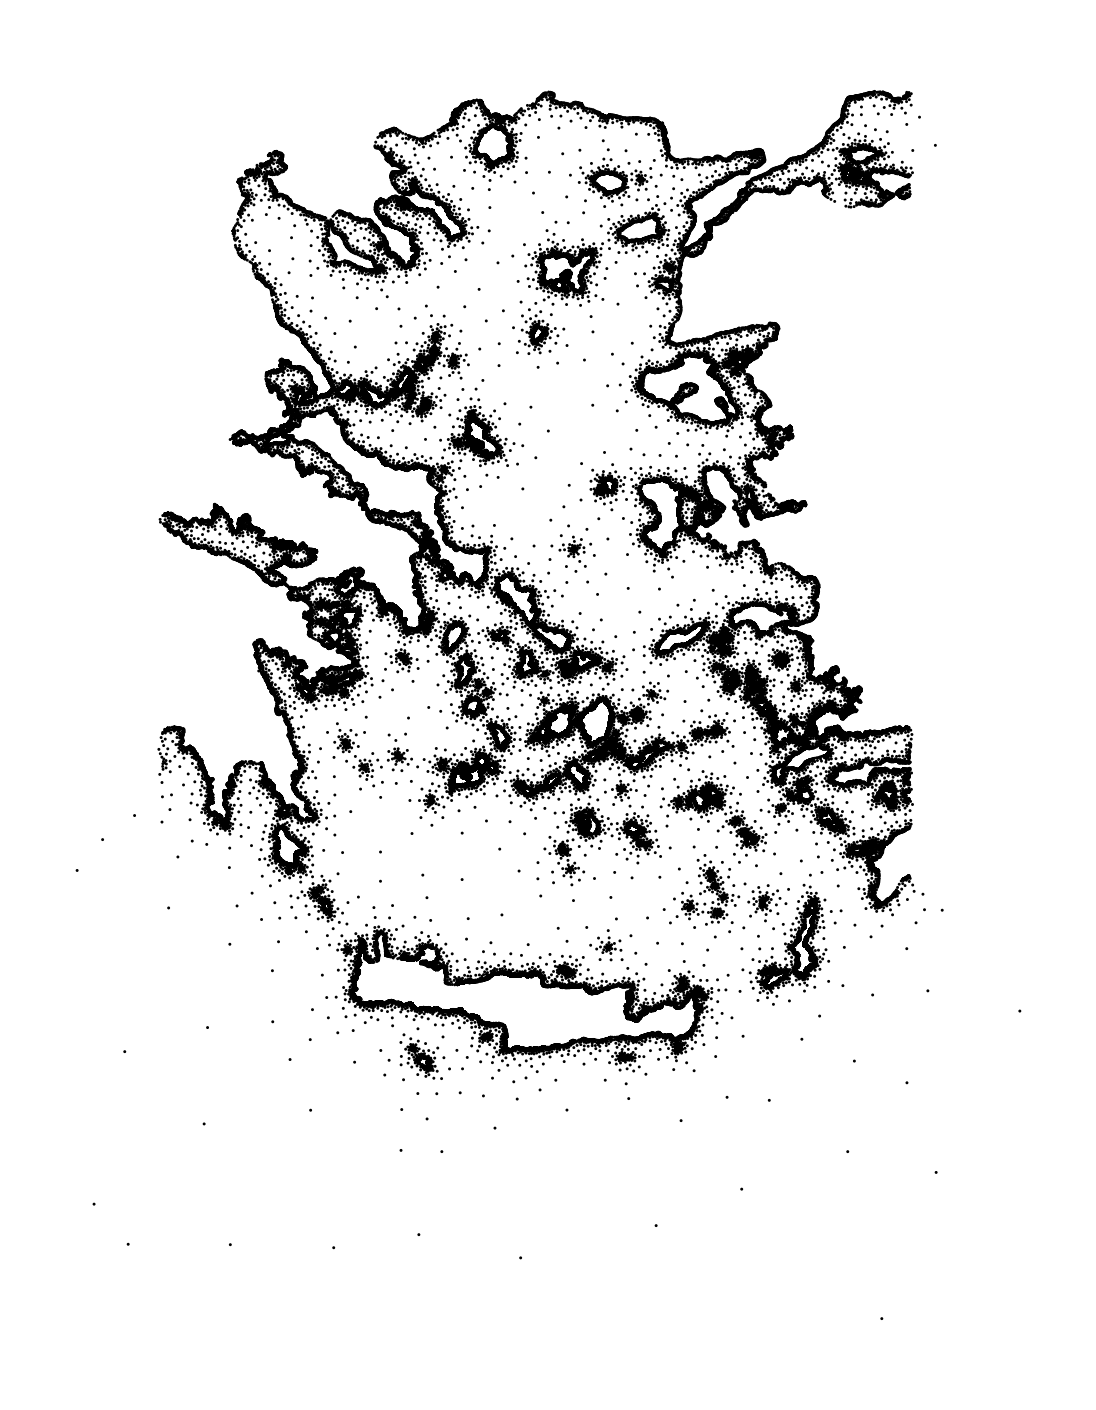
\includegraphics[width=\textwidth]{img/base_graphs/aegaeis-ref-graph.png}
        \caption{aegaeis-graph}
    \end{subfigure}
    \hfill
    \begin{subfigure}[b]{0.35\textwidth}
        \centering
        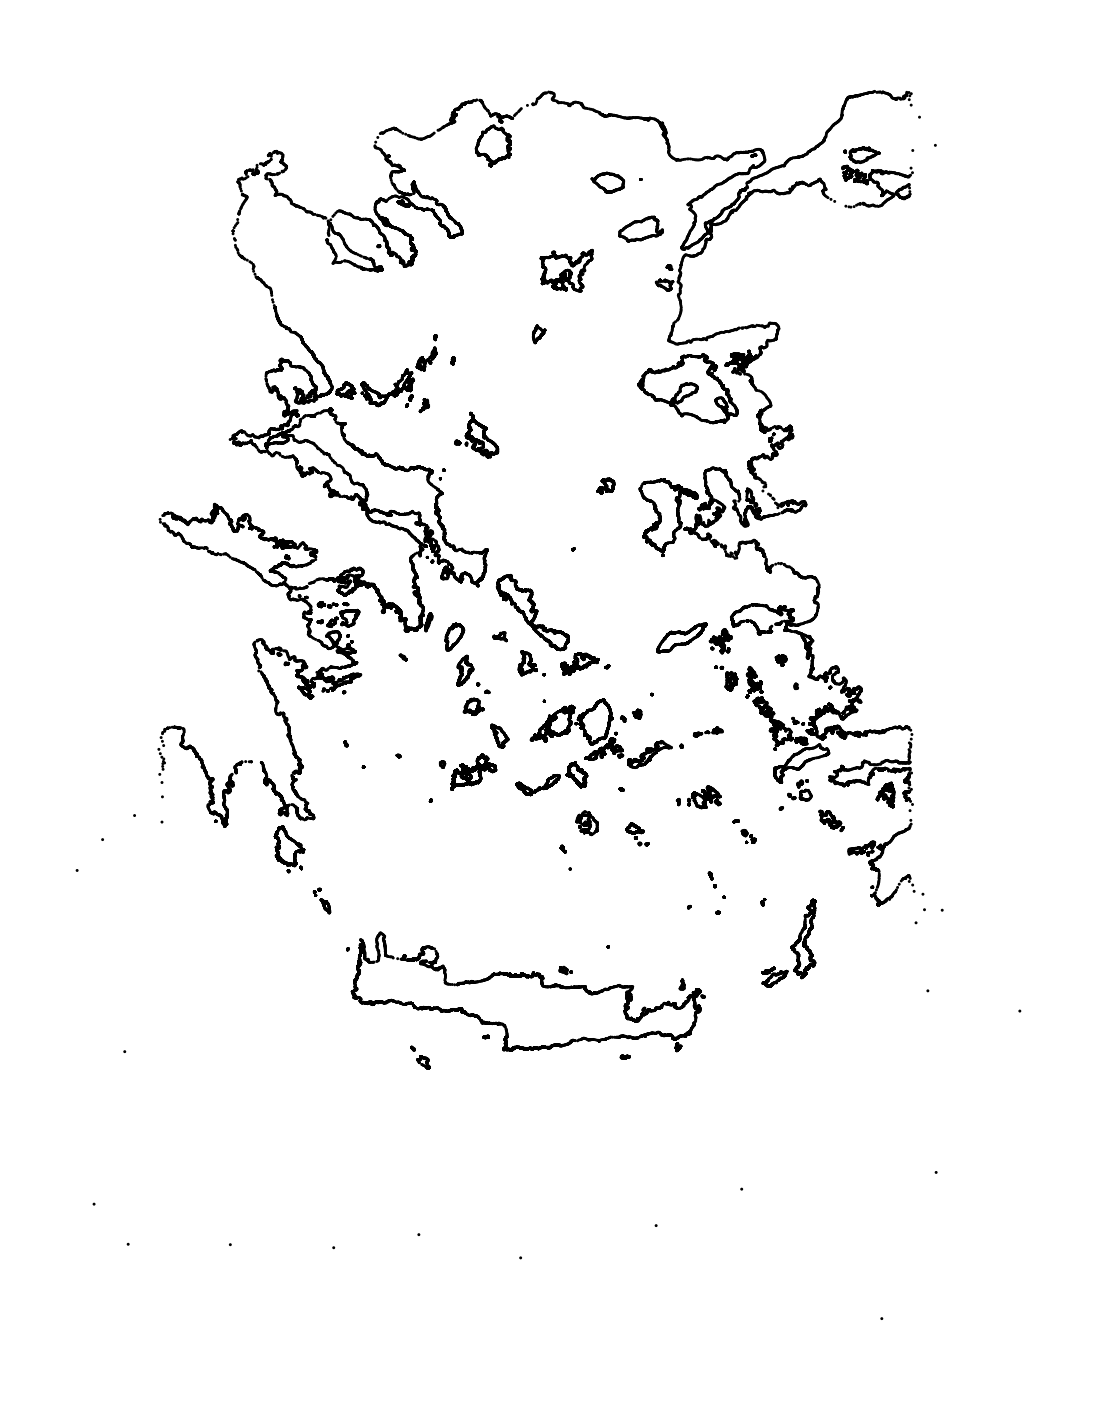
\includegraphics[width=\textwidth]{img/base_graphs/aegaeis-ref-visibility.png}
        \caption{aegaeis-visibility}
    \end{subfigure}
    \\
    \begin{subfigure}[b]{0.35\textwidth}
        \centering
        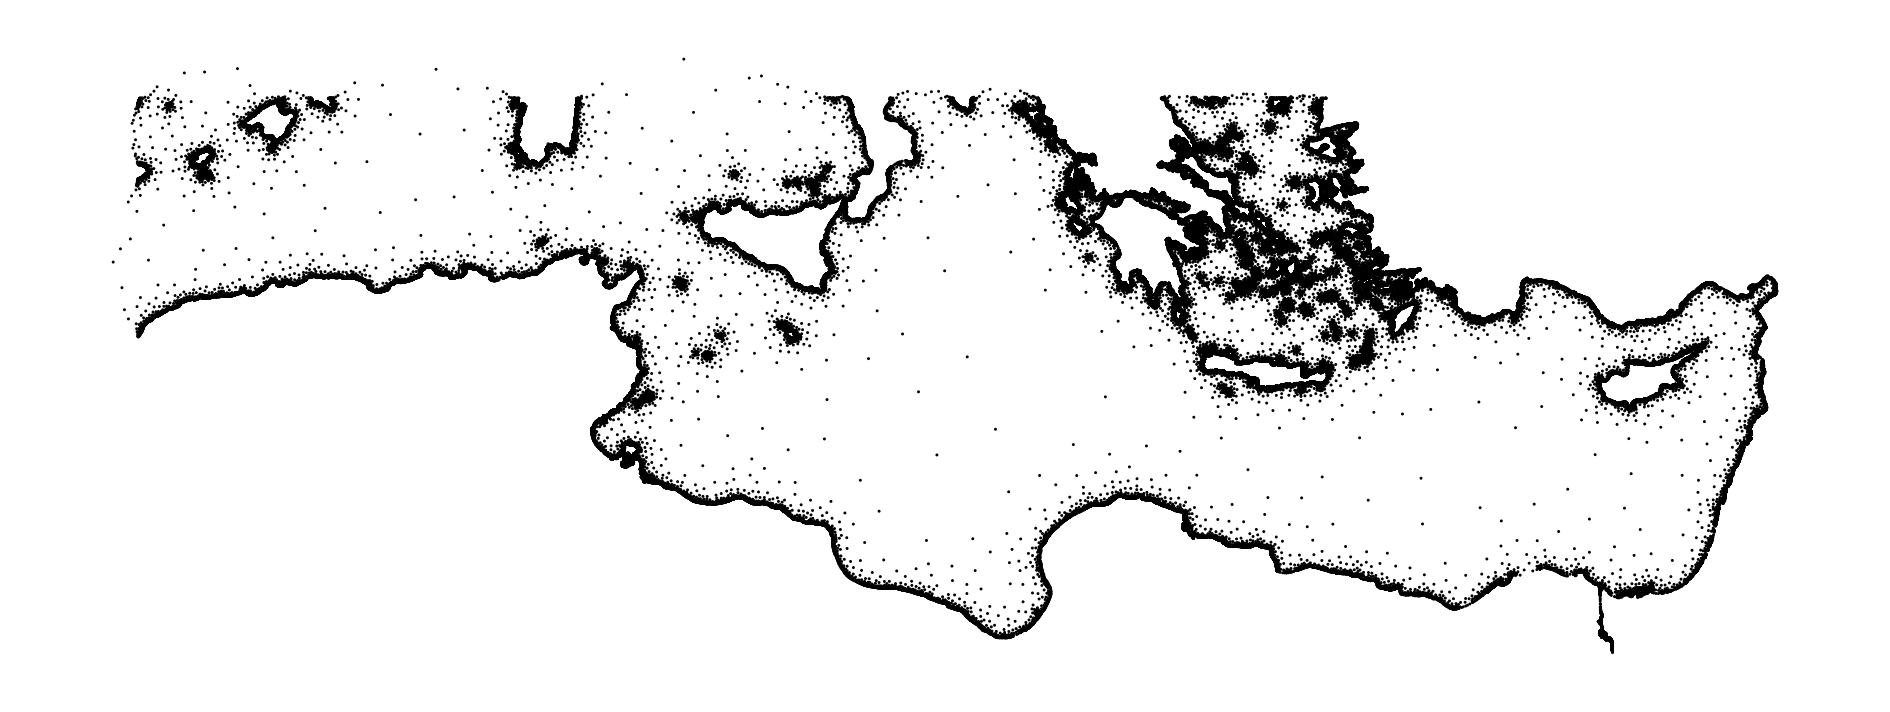
\includegraphics[width=\textwidth]{img/base_graphs/medi-ref-graph.png}
        \caption{medi-graph}
    \end{subfigure}
    \hfill
    \begin{subfigure}[b]{0.35\textwidth}
        \centering
        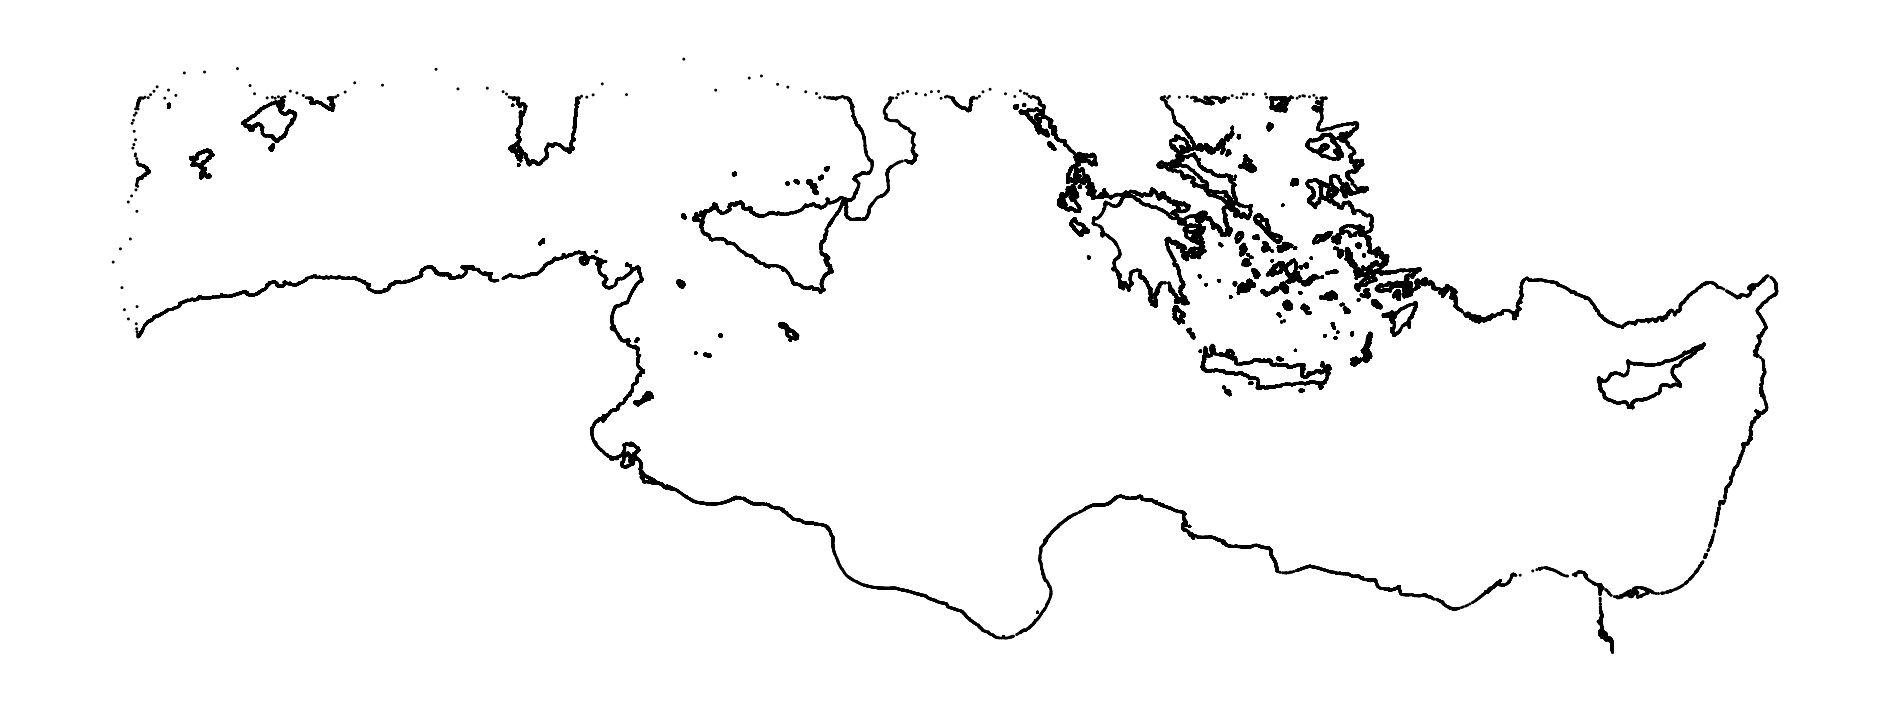
\includegraphics[width=\textwidth]{img/base_graphs/medi-ref-visibility.png}
        \caption{medi-visibility}
    \end{subfigure}
    \\
    \begin{subfigure}[b]{0.35\textwidth}
        \centering
        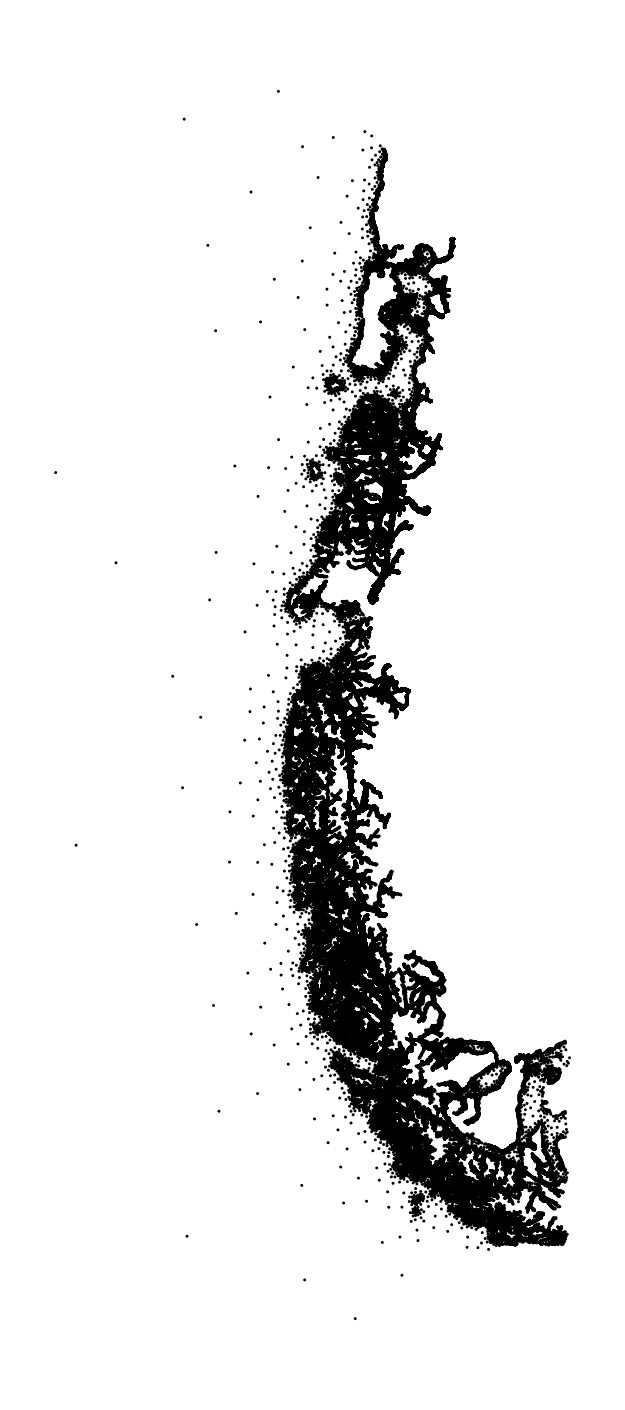
\includegraphics[width=\textwidth]{img/base_graphs/pata-ref-graph.png}
        \caption{pata-graph}
    \end{subfigure}
    \hfill
    \begin{subfigure}[b]{0.35\textwidth}
        \centering
        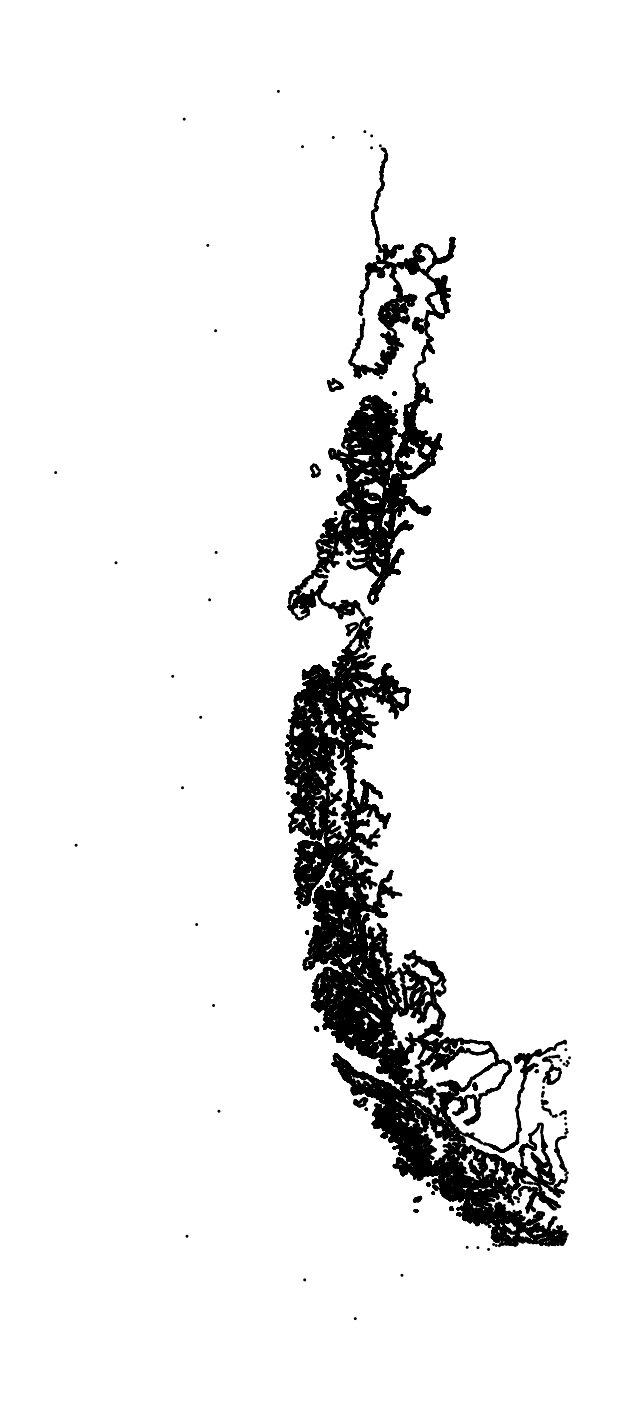
\includegraphics[width=\textwidth]{img/base_graphs/pata-ref-visibility.png}
        \caption{pata-visibility}
    \end{subfigure}
    \caption{Three simple graphs}
    \label{fig:three graphs}
\end{figure}


Sämtlichen Ergebisse wurden im BwUniCluster2.0 erzeugt. Sofern nicht anders erwähnt wurden
2x Intel Xeon Gold 6230
180GB RAM verwendet.


Die bereitgestellten Graphen mussten vor ihrer Nutzung gereinigt und an die Implementierung angepasst werden.
Sie enthielten isolierte Knoten, und die Kantengewichte der Sichtbarkeitsgraphen waren als Gleitkommazahlen gespeichert.
Für die Anpassung wurde ein Python-Skript benutzt, das folgende Aufgaben durchführt:

\begin{itemize}
    \item
          Transformation der Kantengewichte.

    \item
          Entfernung isolierter Knoten.

    \item
          Anpassung der Knoten-IDs, sodass die Knoten-IDs im Sichtbarkeitsgraphen den Bereich $0, \dotsc, n$ und im triangulierten Graphen den Bereich $0, \dotsc, n + m$ umfassen.
\end{itemize}

Während der Untersuchung der triangulierten Graphen wurde festgestellt, dass einige Kanten ein Gewicht von 0 aufwiesen.
Diese Kanten wurden unverändert beibehalten.

medi und pata Sichtbarkeitsgraphen fehlten jeweils einige Kanten, damit sie ungerichtet sind.
Diese wurden von Hand ergänzt.

\todo{Plot degree before after}

\section{Untersuchung der Graphen}

plot edge degree

vergleich der Abstände im vis und graph, sortiert nach hops in vis.




Vielleicht nur n mal insgesammt updaten? alle 10\% neu berechnen?



Heuristic egde difference (zufall)
Vis graphen haben sehr hohen degree (TODO Beweis).
Daher degree x degree viele checks, das gehtn schnell in die Millionen bis Milliarden.
Idee: betrachte nur ein Subset (tails, heads) und schaue ob und wie genau dieses die Edge difference aproximiert.

Das kann dann wieder für andere Methoden benutzt werden.

Plot hitting set vs bottom-up order

\section{Dijkstra}

Als Baseline wurden für jeden Graphen 1000 one-to-one Dijsktra-Suchen squentiell asugeführt. \todo{Darf ich auch parallel}?
Zur Speicherung der Distanzen und Vorgänger wurde ein Vec, als Warteschlange ein BinaryHeap und zum speichern, ob ein Knoten bereits expanded wurde ein BitSet verwendet.
\autoref{ergebnisse::table:dijkstra_one_to_one} zeigt die erzielten Zeiten.
Soweit nicht anders angegeben beziehen sich die Zeit immer auf das finden und erstellen des kürzesten Pfades.

\begin{table}[h]
    \centering
    \begin{tabular}{
            l % Graph
            S[table-format = 4.1] % Zeit
        }
        \toprule
        {Graph}            & {$\varnothing$ t (ms)} \\ \midrule
        aegaeis-graph      & 55.927509              \\
        aegaeis-visibility & 611.561878             \\
        medi-graph         & 93.091061              \\
        medi-visibility    & 1328.95972             \\
        pata-graph         & 245.354415             \\
        pata-visibility    & 964.165614             \\ \bottomrule
    \end{tabular}
    \caption{Dijkstra one-to-one, averaged over 1000 sequential searches}
    \label{ergebnisse::table:dijkstra_one_to_one}
\end{table}

Zusätzlich wurde die Durschnitliche Hop-Länge, Dijsktra Rank und Queue Pops untersucht.

\begin{table}[h]
    \centering
    \begin{tabular}{
            l % Graph
            S[table-format = 3.1] % hop-länge
            S[table-format = 7.0] % rank
            S[table-format = 7.0] % queue pops
        }
        \toprule
        {Graph}            & {Hop-Länge} & {Rank}    & {Queue pops} \\ \midrule
        aegaeis-graph      & 215.7201    & 260447.36 & 325845.56    \\
        aegaeis-visibility & 16.311      & 98650.82  & 517346.63    \\
        medi-graph         & 340.445     & 394855.78 & 494553.97    \\
        medi-visibility    & 23.6149     & 154092.42 & 959206.4     \\
        pata-graph         & 883.979     & 1120841.9 & 1387047.8    \\
        pata-visibility    & 63.817      & 498570.2  & 2429689.8    \\ \bottomrule
    \end{tabular}
    \caption{Dijkstra one-to-one, averaged over 1000 sequential searches}
\end{table}


Es wurde untersucht, ob es sinvoll ist, andere Datenstrukturen zu verwenden, insbesondere eine Warteschlange, die eine \emph{Drecrease-Key} Funktion anbietet.

\section{CH mit Witness}

Es wurde versucht die CH mit Witness, Edge Difference, Lacy Popping zu erstellen.
Dies hat für die Sichtbarkeitsgraphen nicht funktioniert, da 3 Tage nicht ausreichten die Graphen zu erzeugen.
Die Suche ist einfach zu teuer.
Pro Vorgänger muss eine Suche zu allen Nachfolgern gemacht werden.
\todo{Wie teuer ist das in der Ausgangslage?}

\begin{table}[h]
    \centering
    \begin{tabular}{
            l % Graph
            S[table-format = 1.2] % creation zeit
            S[table-format = 4.1] % average time
        }
        \toprule
        {Graph}       & {creation time (min)} & {$\varnothing$ t (µs)} \\ \midrule
        aegaeis-graph & 2.1336                & 514.069                \\
        medi-graph    & 3.08033333333         & 543.803                \\
        pata-graph    & 9.84055               & 730.317                \\\bottomrule
    \end{tabular}
    \caption{ch one-to-one, averaged over 1000 sequential searches}
\end{table}

\section{CH All-In}

All in sortiert nach all in edge differnce:


\section{Hitting Set}

Für die Graphen wurden jeweils ein Hitting Set über \num{100000} Pfade erstellt.
Diese Pfade wurden mit Dijkstra erstellt.

Wie hitbar sind die Graphen? plote hit percentage

\section{CH Bruteforce}

\begin{table}[h]
    \centering
    \begin{tabular}{
            l % Graph
            S[table-format = 1.2] % creation zeit
            S[table-format = 4.1] % average time
        }
        \toprule
        {Graph}            & {creation time (min)} & {$\varnothing$ t (µs)} \\ \midrule
        aegaeis-graph      &                       &                        \\
        aegaeis-visibility &                       &                        \\
        medi-graph         &                       &                        \\
        medi-visibility    &                       &                        \\
        pata-graph         &                       &                        \\
        pata-visibility    &                       &                        \\  \bottomrule
    \end{tabular}
    \caption{ch one-to-one, averaged over 1000 sequential searches}
\end{table}

\section{HL Merge}

Das Merging war deutlicht teruer als erwartet, da ch Kantengrad x HL Label Size

\begin{table}[h]
    \centering
    \begin{tabular}{
            l % Graph
            S[table-format = 1.2] % creation zeit
            S[table-format = 4.1] % average time
        }
        \toprule
        {Graph}            & {creation time (min)} & {$\varnothing$ t (µs)} \\ \midrule
        aegaeis-graph      &                       &                        \\
        aegaeis-visibility &                       &                        \\
        medi-graph         &                       &                        \\
        medi-visibility    &                       &                        \\
        pata-graph         &                       &                        \\
        pata-visibility    &                       &                        \\  \bottomrule
    \end{tabular}
    \caption{hl one-to-one, averaged over 1000 sequential searches}
\end{table}

\section{HL Bruteforce}

\begin{table}[h]
    \centering
    \begin{tabular}{
            l % Graph
            S[table-format = 1.2] % creation zeit
            S[table-format = 4.1] % average time
        }
        \toprule
        {Graph}            & {creation time (min)} & {$\varnothing$ t (µs)} \\ \midrule
        aegaeis-graph      &                       &                        \\
        aegaeis-visibility &                       &                        \\
        medi-graph         &                       &                        \\
        medi-visibility    &                       &                        \\
        pata-graph         &                       &                        \\
        pata-visibility    &                       &                        \\  \bottomrule
    \end{tabular}
    \caption{hl one-to-one, averaged over 1000 sequential searches}
\end{table}

\section{Großes Hitting set}

\section{}
